\chapter{Reducibility of Representations, I}
\label{ch-reducibility1}



This chapter is based on Joshi's book Ref.\cite{Joshi-book}.

Representations (reps) of groups are defined in Section \ref{sec-def-rep}.
In this chapter, we will discuss
 reps of finite groups in more detail.

\section{Symmetries of a Square}

\begin{figure}[h!]
\centering
\includegraphics[width=5in]
{reducibility1/syms-square.png}
\caption{Symmetries of a square.
}
\label{fig-syms-square}
\end{figure}
Fig.\ref{fig-syms-square}
shows an 8 order group $\sqgroup$\footnote{Joshi Ref.\cite{Joshi-book} calls this group $C_{4\nu}$} of symmetries of
a square. The group is generated by the 3 generators
$N_1$, $N_2$ and $S_{2}$. (i.e., every group element is of the form $N_1^a N_2^b S_{12}^c$,
for $a,b,c\in\ZZ_{>0}$.
The operators $N_i$ for $i=1,2$
replace $i$'th component
by its negative. The operator $S_{12}$
swaps components 1 and 2. Ref.\cite{Joshi-book}
uses $m_x=N_2$, $m_y=N_1$, $\s_u=\s_{y=-x}$,
$\s_v=\s_{y=x}$.
$(x,y)$ maps to whatever it says under each square.

\beq
[N_1, N_2]=0, \quad \begin{pmatrix}N_1\\N_2\end{pmatrix}
S_{12}=S_{12}\begin{pmatrix}N_2\\N_1\end{pmatrix}, \quad
N_1^2=N_2^2=S_{12}^2=1
\eeq

Using these simple-to-remember identities,
we could easily calculate a
\qt{multiplication table} for $\sqgroup$.
(i.e. a table with all the elements of the group
as column and row labels, and with 
the product $ab$ as entry 
for row $a$ and column $b$). We won't do so here but
you can find it in Ref.\cite{Joshi-book}.

Conjugacy classes (CC) are defined in Chapter  \ref{ch-lagranges-theorem}.
The CCs of $\sqgroup$ are 
given in Fig.\ref{fig-cc-sqgroup}.
\begin{figure}[h!]
\begin{tabular}{l}
\\ $CC_1=(E)$
\\ $CC_2=(N_1 S_{12}, N_2 S_{12})$ (rotations  by $90$ and $270$ degrees)
\\ $CC_3=(N_1N_2)$ (rotation by 180 degrees)
\\ $ CC_4=(N_1, N_2)$ (refection about $x$ or $y$ axis)
 \\ $CC_5=(S_{12}, N_1N_2 S_{12})$ (reflection about $y=x$ or $y=-x$ diagonals)
\end{tabular}
\caption{CCs for $\sqgroup$}
\label{fig-cc-sqgroup}
\end{figure}

\begin{table}[h!]
\begin{tabular}{|l|
>{\columncolor[HTML]{CBCEFB}}l |
>{\columncolor[HTML]{FFFFC7}}l |
>{\columncolor[HTML]{FFFFC7}}l |
>{\columncolor[HTML]{96FFFB}}l |
>{\columncolor[HTML]{FFCCC9}}l |
>{\columncolor[HTML]{FFCCC9}}l |
>{\columncolor[HTML]{9AFF99}}l |
>{\columncolor[HTML]{9AFF99}}l |}
\hline
 & $E$ & $C_4$ & $C_4^3$ & $C_4^2$ & $N_2$ & $N_1$ & $\s_{y=-x}$ & $\s_{y=x}$ \\ \hline
$\rho^{(1)}$ & 1 & 1 & 1 & 1 & 1 & 1 & 1 & 1 \\ \hline
$\rho^{(2)}$ & 1 & --1 & --1 & 1 & --1 & --1 & 1 & 1 \\ \hline
$\rho^{(3)}$ & 1 & --1 & --1 & 1 & 1 & 1 & --1 & --1 \\ \hline
$\rho^{(4)}$ & 1 & 1 & 1 & 1 & --1 & --1 & --1 & --1 \\ \hline
$\rho^{(5)}$ 
& $\begin{pmatrix}1&0\\0&1 \end{pmatrix}$
& $\begin{pmatrix}0&-1\\1&0 \end{pmatrix}$
& $\begin{pmatrix}0&1\\-1&0 \end{pmatrix}$
& $\begin{pmatrix}-1&0\\0&-1 \end{pmatrix}$
& $\begin{pmatrix}1&0\\0&-1 \end{pmatrix}$
& $\begin{pmatrix}-1&0\\0&1 \end{pmatrix}$
& $\begin{pmatrix}0&-1\\-1&0 \end{pmatrix}$
& $\begin{pmatrix}0&1\\1&0 \end{pmatrix}$ 
\\ \hline
\end{tabular}
\caption{Irreps of $\sqgroup$. Different color for each CC.
Number of inequivalent irreps = number 
of CCs.}
\label{tab-sq8-irreps}
\end{table}

\begin{table}[h!]
\begin{tabular}{|l|
>{\columncolor[HTML]{CBCEFB}}l |
>{\columncolor[HTML]{FFFFC7}}l |
>{\columncolor[HTML]{FFFFC7}}l |
>{\columncolor[HTML]{96FFFB}}l |
>{\columncolor[HTML]{FFCCC9}}l |
>{\columncolor[HTML]{FFCCC9}}l |
>{\columncolor[HTML]{9AFF99}}l |
>{\columncolor[HTML]{9AFF99}}l |}
\hline
 & $E$ & $C_4$ & $C_4^3$ & $C_4^2$ & $N_2$ & $N_1$ & $\s_{y=-x}$ & $\s_{y=x}$ \\ \hline
$\chi^{(1)}$ & 1 & 1 & 1 & 1 & 1 & 1 & 1 & 1 \\ \hline
$\chi^{(2)}$ & 1 & --1 & --1 & 1 & --1 & --1 & 1 & 1 \\ \hline
$\chi^{(3)}$ & 1 & --1 & --1 & 1 & 1 & 1 & --1 & --1 \\ \hline
$\chi^{(4)}$ & 1 & 1 & 1 & 1 & --1 & --1 & --1 & --1 \\ \hline
$\chi^{(5)}$ 
& 2
& 0
& 0
& --2
& 0
& 0
& 0
& 0
\\ \hline
\end{tabular}
\caption{Characters of $\sqgroup$. Different color for each CC.
$\chi^\alp(g)=\tr\rho^\alp$ for all
$g\in \calg$.
Check that $\sum_{g\in\calg}\chi^\alp(g)
\chi^{\beta*}(g)=|\calg|\delta_{\alp\beta}$.
}
\label{tab-sq8-char}
\end{table}



\section{Block Diagonalization}
Rearrangement theorem: $aG=a$ for a group $G$ and 
$a\in G$.



Suppose $S$ (smaller) and $L$ (larger) are two vector spaces and $S\subset L$, with $L\neq S$ (i.e., proper subspace). Suppose $\calg$ is a group.
Suppose $\calg S\subset S$ and $\calg L  \subset L$. Then  we say $S$ is an
{\bf invariant subspace} of $L$ under $\calg$,
and we say  $L$ is {\bf reducible} under $\calg$.



\begin{claim}
Suppose $S$ is an invariant subspace of $L$ under $\calg$. Then for any rep $(L, \rho_L)$ of $\calg$, we must have

\beq
\rho_L(g)=
\begin{array}{r|cc}
&S&S^c
\\
\hline
S&A^{d_S\times d_S}&0
\\S^c&C^{d_{S^c}\times d_S}& D^{d_{S^c}\times d_{S^c}}
\end{array}
\label{eq-redu-mat}
\eeq
for all $g\in \calg$,
where $S^c=L-S$, $d_S=$ dimension of vector space $S$, $d_{S^c}=$ dimension of vector space $S^c$.
Furthermore, if $\rho_L()$ is a unitary rep,
then

\beq
C^{d_{S^c}\times d_S}=0
\eeq


\end{claim}
\proof

The zero matrix in \ref{eq-redu-mat}
follows because $\calg S\subset S$.
Note that 
if

\beq
\rho_L(g_1)=
\begin{pmatrix}
A_1&0
\\
C_1&D_1
\end{pmatrix},\quad
\rho_L(g_2)=
\begin{pmatrix}
A_2&0
\\
C_2&D_2
\end{pmatrix}
\eeq
then

\beq
\rho_L(g_1)\rho_L(g_2)=
\begin{pmatrix}
A_1 A_2&0
\\
X & D_1 D_2
\end{pmatrix}
\eeq
where

\beq X=C_1 A_2 + D_1 C_2 \eeq
If
$\rho()$ is a unitary rep,
then $X=0$ because the rows of 
the full matrix must yield $d_L$
orthonormal vectors and the columns must too.
This is possible only if $X=0$.

If $X=0$, we can define unitary reps $\rho_S$ and $\rho_{S^c}$ so that

\beq
\rho_S(g_1)=A_1,\quad \rho_S(g_2)=A_2,\quad
\rho_S(g_1 g_2)=A_1 A_2
\eeq

\beq
\rho_{S^c}(g_1)=D_1,\quad \rho_{S^c}(g_2)=D_2,\quad
\rho_{S^c}(g_1 g_2)=D_1 D_2
\eeq
\qed

\begin{claim}
For any representation $\rho()$,
there is an equivalent unitary rep $\hat{\rho}()$.
\end{claim}
\proof

Define the Hermitian matrix $H$ by

\beq
H=\sum_{g\in\calg}\rho(g)\rho^\dagger(g)
\eeq

Find a unitary matrix $U$ that diagonalizes $H$:

\beqa
H_d &=& U^\dagger H U
\\
&=&
U^\dagger\left[
\sum_{g\in\calg}\rho(g)\rho^\dagger(g)
\right]
U
\eeqa
where $H_d$ is a diagonal matrix.


Define a new rep $\rho_1()$ by

\beq
\rho_1(g)= U^\dagger \rho(g) U
\eeq
for all $g\in\calg$.

Note that  
\beq
H_d =\sum_{g\in\calg }\rho_1(g)\rho_1^\dagger(g)
\eeq

Note that the diagonal elements of $H_d$
must be positive.
Indeed,

\beqa
(H_d)_{kk} &=&
 \sum_{g\in\calg}\sum_j
\rho_1(g)_{kj}\rho_1^*(g)_{kj}
\\\
&=&
\sum_{g\in\calg}\sum_j 
\left|\rho_1(g)_{kj}\right|^2
\\
&\geq& 0
\eeqa
Actually, the diagonal elements of
$H_d$ must be strictly positive
because if the $k$th one were zero,
the $k$ row of $\rho_1(g)$ would be zero
for all $g\in\calg$. So all 
$\rho_1(g)$ would have a zero
determinant. 
Then all $\rho(g)$
would have a zero determinant and no inverse.
Then the rep $\rho()$
that we started would not
be valid, in contradiction
with the premise of the claim.

Now define

\beq
\hat{\rho}(g)=
H_d^{-\frac{1}{2}}
\rho_1(g)H_d^{\frac{1}{2}}
\eeq
for $g\in \calg$. 

Finally, check that $\hat{\rho}(g)$ is unitary
for all $g\in\calg$.

\beqa
\hat{\rho}(g)
\hat{\rho}^\dagger(g)
&=&
H_d^{-\frac{1}{2}}
\rho_1(g)
H_d
\rho_1^\dagger(g)
H_d^{-\frac{1}{2}}
\\
&=&
H_d^{-\frac{1}{2}}
\rho_1(g)
\left[
\sum_{g'\in\calg }\rho_1(g')\rho_1^\dagger(g')
\right]
\rho_1^\dagger(g)
H_d^{-\frac{1}{2}}
\\
&=&
H_d^{-\frac{1}{2}}
\left[
\sum_{g'\in\calg }\rho_1(gg')\rho_1^\dagger(gg')
\right]
H_d^{-\frac{1}{2}}
\\
&=&
H_d^{-\frac{1}{2}}
\left[
H_d
\right]
H_d^{-\frac{1}{2}}
\\
&=& 1
\eeqa
\qed

For any square matrices $A$, $B$, $C$ (not necessarily of the same dimension)
\beq
A\oplus B\oplus C = \begin{pmatrix}
A&0&0
\\0&B&0
\\
0&0&C
\end{pmatrix}
\eeq
If $A_i$ for $i=1,2, \ldots, n$ are square matrices, $A_1\oplus A_2 \oplus \ldots \oplus A_n$ is called
a {\bf block diagonal matrix}.

\beq
\rho(g)=
\bigoplus_\alp x_\alp \rho_\alp(g)
\eeq
where $x_\alp\in \ZZ_{>0}$.

\section{Schur's 2 Lemmas}

\begin{claim}(Schur's Lemma 1)

If $\rho()$ is  an irrep of group $\calg$ and
matrix $P$ satisfies

\beq
\rho(g)P=P\rho(g)
\eeq
for all $g\in \calg$, then

\beq
P=c I
\eeq
where  $I$ is the
unit matrix and $c\in \CC$.
\end{claim}
\proof


Note that 

\beq
P\rho(g)= \rho(g)P \quad \forall g\in\calg
\eeq
implies
\beq
\underbrace{\rho^\dagger(g)}_{\rho(g^{-1})}P^\dagger= P^\dagger\underbrace{\rho^\dagger(g)}_{\rho(g^{-1})}
\quad \forall g\in\calg
\eeq
which implies

\beq
P^\dagger \rho(g)=\rho(g)P^\dagger 
\quad \forall g\in\calg
\eeq
Define

\beq
H= PP^\dagger
\eeq
$H$ is Hermitian and
satisfies

\beq
H\rho(g)=\rho(g)H
\eeq
If we can prove that $H$ is a constant 
matrix, then $P$ must be
a  constant matrix too.
Since $H$ is Hermitian, it must be diagonalizable.
Let

\beq
H\ket{h_j}=h_j\ket{h_j}
\eeq
for $j=1,2, \ldots, n$.
Then

\beq
H\rho(g)=\rho(g)H\implies
(h_i-h_j)\av{h_i|\rho(g)|h_j}=0
\eeq
Hence, if $h_i\neq h_j$ for some $i,j$,
then the matrix $\rho(g)$ 
can be block diagonalized for all $g$.
So as not to contradict the premise that $\rho()$
is an irrep, we are forced to
conclude that all $h_i$ must be equal.
Hence $H$ is indeed a constant matrix.


\qed


\begin{claim}(Schur's Lemma 2)
 
If $\rho_1()$ and $\rho_2()$ 
are two irreps of a group $\calg$ and matrix $M_{12} $ (possibly rectangular) satisfies

\beq
\rho_1(g)M_{12} =M_{12} \rho_2(g)
\eeq
for all $g\in\calg$, then
$M_{12} =0$ or $M_{12} $ is a square matrix with $\det M_{12} \neq 0$. In the latter case,
$\rho_1$ and $\rho_2$ are  equivalent reps.
\end{claim}
\proof

\beq
M_{12} ^\dagger\underbrace{\rho_1^\dagger(g)}
_{\rho_1(g^{-1})}=
\underbrace{\rho_2^\dagger(g)}_{\rho_2(g^{-1})}
M_{12} ^\dagger
\quad \forall g\in\calg
\eeq

\beq
M_{12} ^\dagger\rho_1(g) = \rho_2(g)M_{12} ^\dagger 
\quad \forall g\in\calg
\eeq

\beqa
\rho_1(g)M_{12} M_{12} ^\dagger &=& M_{12} \rho_2(g)M_{12} ^\dagger 
\\
&=&
M_{12} M_{12} ^\dagger\rho_1(g)
\eeqa



\beqa
\rho_2(g)M_{12} ^\dagger M_{12}  &=& M_{12} ^\dagger \rho_1(g)M_{12} 
\\
&=&
M_{12} ^\dagger M_{12} \rho_2(g)
\eeqa

\beq
M_{12} M_{12} ^\dagger = c, 
\quad M_{12} ^\dagger M_{12} = c'
\eeq

Let $d_i$ for $i=1,2$ be
the matrix dimension of $\rho_i$.

\hrule
Assume first that $d_1=d_2=n$.
Then 

\beq
c^n=\det(M_{12} M_{12}^\dagger)=\det(M_{12})\det(M_{12}^\dagger)
\eeq

\begin{itemize}
\item if $c\neq 0$:

Then $\det M_{12}\neq 0$ so $M_{12}$ is
invertible.
Hence 

\beq
M_{12}^{-1} \rho_1(g) M_{12}= \rho_2(g)
\eeq
for all $g\in \calg$. Thus, $\rho_1$ and
$\rho_2$ are equivalent reps.

\item if $c=0$:

Then 
 

\beqa
\sum_j \av{i|M_{12}|j}\av{j|M_{12}^\dagger|i}
&=&
\sum_j|\av{i|M_{12}|j}|^2
\\
&=& 0
\eeqa
so the $i$th row of $M_{12}$ equals zero
for all $i$. Hence we must have $M_{12}=0$.

\end{itemize}
\hrule
When $d_1\neq d_2$, we must have $M_{12}=0$.
This is why.

For simplicity, we will first assume $(d_1, d_2)=(1,2)$
or $(d_1, d_2)=(2,1)$.
In this case, $M$ equals either
a column vector $x=\begin{pmatrix}x_1\\x_2\end{pmatrix}$
or a row vector $x^\dagger$.
Either way we must have

\beq
x x^\dagger = \begin{pmatrix}x_1\\x_2\end{pmatrix}
\begin{pmatrix}x_1^*&x_2^*\end{pmatrix}=c
\label{eq-x-xdag-c}
\eeq
for some constant $c\in \CC$.
This is only possible if

\beq
x_1=x_2=c=0
\eeq
In the general case, when $d_1<d_2$ or $d_2<d_1$,
$M$, $x_1$ is a  square matrix and $x_2$
is  rectangular one. Eq.(\ref{eq-x-xdag-c})
becomes 

\beq
x x^\dagger = \begin{pmatrix}x_1\\x_2\end{pmatrix}
\begin{pmatrix}x_1^\dagger&x_2^\dagger\end{pmatrix}=c
\eeq
This implies $x_1 x_1^\dagger = c$ so, if $c\neq 0$,  
$x_1/\sqrt{c}$ is a unitary matrix and therefore invertible. Since also $x_2 x^\dagger_1=0$,
we must have $x_2=0$. But $x_2 x_2^\dagger =c$ 
so $c=0$. Contradiction.


\qed

\section{ Orthogonality of Irreps}
\begin{claim}
If $\rho_\alp$ and $\rho_\beta$ are 
two irreps of group $\calg$, then

\beq
\begin{array}{l}
\myboxed{
\frac{1}{|\calg|}\sum_{g\in \calg}
\rho_\alp(g)_{ij} 
\underbrace{\rho_\beta(g^{-1})_{j'i'}}
_{=\rho_\beta^\dagger(g)_{j'i'}=\rho_\beta^*(g)_{i'j'}}=
\delta_{\alp \beta}
\delta_{ii'}\frac{\delta_{jj'}}{d_\alp}
}
\\
\frac{1}{|\calg|}\sum_{g\in\calg}
\bcen
\xymatrix@R=1pc@C=1pc{
&\alp&
\\
i&\ar[l]\rho_\alp(g)\ar@{~}[u]&\ar[l]j
}
\ecen
\bcen
\xymatrix@R=1pc@C=1pc{
&\beta&
\\
j'&\ar[l]\rho_\beta(g)\ar@{~}[u]&\ar[l]i'
}
\ecen
=
\frac{1}{d_\alp}
\bcen
\xymatrix@R=.5pc{
\alp&\ar@{~}[l]|\bullet\beta
\\
j&\ar[l]|\bullet j'
\\
i&\ar[l]|\bullet i'
}
\ecen
\end{array}
\label{eq-ortho-irreps}
\eeq
where $d_\alp$ is
the matrix dimension of  $\rho_\alp$
\end{claim}
\proof

As a preliminary sanity check,
note that if we set $\alp=\beta$,
$j=j'$ and we sum over $j$,
both sides yield $\delta_{ii'}$.

Define
\newcommand{\Mab}[0]{M_{\alp\beta}}
\newcommand{\Maa}[0]{M_{\alp\alp}}

\beq
\Mab= \frac{1}{|\calg|}
\sum_{g\in\calg}\rho_\alp(g)X\rho_\beta(g^{-1})
\eeq
where $X$ is some arbitrary matrix.
\hrule
First assume $\rho_\alp\neq \rho_\beta$.

Then

\beqa
\rho_\alp(h)\Mab
&=&
\frac{1}{|\calg|}
\sum_{g\in\calg}\rho_\alp(hg)X\rho_\beta(
(\underbrace{g}_{h^{-1}hg})^{-1})
\\
&=&
\frac{1}{|\calg|}
\sum_{g\in\calg}\rho_\alp(hg)X\rho_\beta(
(hg)^{-1})\rho_\beta(
h)
\\
&=&
\Mab\rho_\beta(h)
\eeqa
for all $h\in\calg$.
Since $\rho_\alp\neq \rho_\beta$,
by Schur's second lemma, 

\beq
\Mab=0
\eeq
The last equation in component form is

\beq
 \frac{1}{|\calg|}
\sum_{g\in\calg}
\sum_{k,k'}
\rho_\alp(g)_{ik}
X_{kk'}
\rho_\beta(g^{-1})_{k'i'}=0
\eeq
Now setting 

\beq
X_{k k'}=\delta_{k j}\delta_{k'j'}
\eeq
we get 

\beq
\frac{1}{|\calg|}
\sum_{g\in\calg}
\rho_\alp(g)_{ij}
\rho_\beta(g^{-1})_{j'i'}=0
\eeq
\hrule
Next assume $\rho_\alp=\rho_\beta$.

Then

\beq
\rho_\alp(h)\Maa
=
\Maa\rho_\alp(h)
\eeq
for all $h\in \calg$, so by Schur's first lemma,

\beq
\Maa=cI
\eeq
Taking the  trace of both sides
of the last equation, we get
\beq
\tr(X)=cd_\alp
\eeq
so

\beq
\Maa = \frac{\tr(X)}{d_\alp}I
\eeq
The last equation in component form is

\beq
 \frac{1}{|\calg|}
\sum_{g\in\calg}
\sum_{k,k'}
\rho_\alp(g)_{ik}
X_{kk'}
\rho_\alp(g^{-1})_{k'i'}=\frac{\tr(X)}{d_\alp}\delta_{ii'}
\eeq

Now setting 

\beq
X_{k k'}=\delta_{k j}\delta_{k'j'},
\quad  \tr(X)=\delta_{jj'}
\eeq
we get 

\beq
\frac{1}{|\calg|}
\sum_{g\in\calg}
\rho_\alp(g)_{ij}
\rho_\alp(g^{-1})_{j'i'}=
\frac{\delta_{jj'}}{d_\alp}\delta_{ii'}
\eeq


\qed
\section{Orthogonality  of Characters}

\beq
\chi^\alp(g)=\tr(\rho^\alp(g))=\sum_k
\rho^\alp(g)_{kk} 
\eeq


$
\tr(AB)=\tr(BA)
$



\beq
\tr(\rho^\alp(hgh^{-1}))=
\tr(\rho^\alp(h)\rho^\alp(g)\rho^\alp(h^{-1}))=\tr\rho^\alp(g)
\eeq
\beq
\chi^\alp(hgh^{-1})=\chi^\alp(g)
\eeq

$g(CC_k)=$ one candidate of the conjugacy
class $CC_k$.

\beq
\chi^\alp_k=\chi^\alp(g(CC_k))=\chi^\alp(g)
\eeq
for $g\in CC_k$.



\begin{claim}

\beq
\frac{1}{|\calg|}
\sum_{g\in \calg}
\chi^\alp(g)\chi^{\beta *}(g)
=\delta_{\alp\beta}
\label{eq-ortho-char}
\eeq

\beq
\frac{1}{|\calg|}
\sum_{k=1}^{N_{CC}}|CC_k|\;
\chi^\alp_k\;\chi^{\beta *}_k
=\delta_{\alp\beta}
\eeq

\end{claim}
\proof

Setting $i=j$ and $i'=j'$ in Eq.\ref{eq-ortho-irreps},
we get

\beq
\frac{1}{|\calg|}\sum_{g\in \calg}
\rho_\alp(g)_{ii} 
\rho_\beta(g^{-1})_{i'i'}
=
\delta_{\alp \beta}
\delta_{ii'}\frac{\delta_{ii'}}{d_\alp}
\eeq
Now summing both sides over $i$ and $i'$
gives Eq.\ref{eq-ortho-char}.

\qed

multiplication of classes

\beq
CC_i CC_j =\{ ab\mid a\in CC_i, b\in CC_j\}
\eeq

\beq
CC_i CC_j =\sum_k a^k_{ij}CC_k
\eeq
where $a^k_{ij}\in \ZZ_{>0}$.

\begin{claim}
If 

\beq
CC_i\; CC_j =\sum_k a_{ijk}CC_k
\eeq
then



\beq
|CC_i|\;|CC_j|\chi^\alp_i
\chi^\alp_j
=
d_\alp\sum_k a_{ijk}|CC_k|\chi^\alp_k
\eeq
\end{claim}
\proof

\beq
\rho^\alp_k=
\sum_{g\in CC_k}\rho^\alp(g)
\eeq


\beqa
\rho^\alp(g)
\rho^\alp_k
\rho^\alp(g^{-1})
&=&
\sum_{g_1\in CC_k}
\rho^\alp(g)
\rho^\alp(g_1)
\rho^\alp(g^{-1})
\\
&=&
\sum_{g_1\in CC_k}
\rho^\alp(gg_1g^{-1})
\\
&=&
\rho^\alp_k
\eeqa

\beq
\rho^\alp_k = c^\alp_k I
\eeq

\beq
|CC_k|\chi^\alp_k=c^\alp_kd_\alp
\eeq

\beq
\rho^\alp_k=\frac{|CC_k|}{d_\alp}\chi^\alp_k I
\eeq

\beqa
\rho^\alp_i \rho^\alp_j
&=&
\sum_{g_1\in CC_i}\sum_{g_2\in CC_j}
\rho^\alp(g_1 g_2)
\\
&=&\sum_{g\in CC_i \;CC_j}\rho^\alp(g)
\\
&=&
\sum_k a_{ijk}\sum_{g\in CC_k}\rho^\alp(g)
\\
&=&
\sum_k a_{ijk}\rho^\alp_k
\eeqa

\beq
\frac{|CC_i|}{d_\alp}\chi^\alp_i
\frac{|CC_j|}{d_\alp}\chi^\alp_j 
=
\sum_{k}a_{ijk}
\frac{|CC_k|}{d_\alp}\chi^\alp_k 
\eeq

\qed

\begin{claim}
Suppose\footnote{Recall that we define
$A\equiv B$ , $A$ is equivalent to $B$,
if they 
are equal up to a similarity transformation.}

\beq
\rho(g) \equiv\bigoplus_\alp m_\alp \rho^\alp(g)
\eeq
for all $g\in\calg$
where $m_\alp\in \ZZ_{>0}$
and the $\rho_\alp$ are distinct irreps.
Then

\beq
\chi(g)=
\sum_\alp m_\alp \chi^\alp(g)
\eeq
for all $g\in \calg$. Furthermore,

\beq
\frac{1}{|\calg|}
\sum_{g\in \calg}
\chi^{\alp*}(g)\chi(g)
= m_\alp
\eeq

\beq
\frac{1}{|\calg|}\sum_{g\in\calg}
\chi^*(g)\chi(g)=
\sum_\alp  |m_\alp|^2
\label{eq-m-alp-sq}
\eeq

\end{claim}
\proof

\beqa
\sum_{g\in \calg}\chi^{\alp*}(g)\chi(g)
&=&
\sum_\beta m_\beta \sum_{g\in \calg}
\chi^{\alp*}(g)\chi^\beta(g)
\\
&=&
m_\alp |\calg|
\eeqa

\beqa
\frac{1}{|\calg|}\sum_{g\in\calg}
\chi^*(g)\chi(g)
&=&
\frac{1}{|\calg|}
\sum_\alp \sum_\beta m_\alp^* m_\beta
\sum_{g\in \calg}
\chi^{\alp*}(g)
\chi^\beta(g)
\\
&=&
\sum_\alp  |m_\alp|^2
\eeqa

\qed

\begin{claim}
The rep $\rho$ of group $\calg$ 
is irreducible iff

\beq
\sum_{g\in\calg}
\chi^*(g)\chi(g)
=|\calg|
\eeq
or, equivalently,

\beq
\sum_k |CC_k|\;\chi^*_k \chi_k=|\calg|
\eeq
where $\chi(g)=\tr (\rho(g))$
and $\chi_k = \chi(g(CC_k))$.
\end{claim}
\proof

This claim follows
from Eq.(\ref{eq-m-alp-sq})
with $m_\alp=1$ for a single 
irrep $\alp$.

\qed


Regular rep

\beq
\rho^{reg}(g)_{g_1, g_2}=
\indi(g=g_1^{-1}g_2)=\delta_{g, g^{-1}_1g_2}
\eeq
The regular rep for 
any $g\in\calg$
is a $|\calg|\times |\calg|$
matrix with each row and column being one-hot\footnote{A one-hot vector
has all its components equal to
zero except one component equal to one.}.
That's because given $(g, g_1)$, there is only one $g_2$ for which $g=g_1^{-1}g_2$.
Likewise, given one $(g, g_2)$,
there is only one suitable $g_1$.
Note also that

\beq
\rho^{reg}(g)_{g_1, g_1}=\delta_{g, e}, \quad \chi^{reg}(g)=\delta_{g,e}|\calg|
\eeq
for all $g\in \calg$.


\beqa
\sum_{g_2}\rho^{reg}(a)_{g_1, g_2}
\rho^{reg}(b)_{g_2, g_3}
&=&
\sum_{g_2}
\delta_{a, g_1^{-1}g_2}
\delta_{b, g_2^{-1} g_3}
\\
&=&
\delta_{a , g_1^{-1}(  g_3b^{-1})}
\\
&=&
\delta_{ab, g_1^{-1}g_3}
\\
&=&
\rho^{reg}(ab)
\eeqa

\begin{claim}

\beq
\chi^{reg}=\sum_\alp d_\alp \chi^\alp
\eeq

\beq
|\calg|=\sum_\alp d^2_\alp
\eeq
\proof
 \beq
\rho^{reg}\equiv\bigoplus_\alp m_\alp \rho^\alp
\eeq


\beqa
m_\alp
&=&
\frac{1}{|\calg|}
\sum_{g\in\calg}
\chi^{\alp*}(g)
\underbrace{\chi_{rep}(g)}_{\delta_{g,e}|\calg|}
\\
&=&
\underbrace{\chi^{\alp*}(e)}_{d_\alp}
\eeqa

\qed

\end{claim}



\section{More Reps}
\begin{enumerate}
\hrule
\item (plane wave rep 8-dim rep of $\sqgroup$)

$\vec{r} = (p_1x_1,p_2x_2)$

$\vec{k}=(k_1, k_2)$


$(G_a)_{a=1}^8=(E, C_4, C_4^3, C_4^2, N_2, N_1, \s_{y=-x}, \s_{y=x})$

$\vec{r}_a = G_a\vec{r}$

$G_a\ket{\vec{r}}=\ket{G_a\vec{r}}=\ket{\vec{r}_a}$


\beq
\av{\vec{k}|\phi_a(\vec{r})}=
\av{\vec{k}|\vec{r}_a}=
\exp(i\vec{k}\cdot \vec{r}_a)
\eeq

\beqa
\av{\vec{r}_{a_1}|\vec{r}_{a_2}}
&=&\int \frac{d^2k}{(2\pi)^2}
\av{\vec{r}_{a_1}|\vec{k}}
\av{\vec{k}|\vec{r}_{a_2}}
\\
&=&
\delta(\vec{r}_{a_1}-\vec{r}_{a_2})
\eeqa

\beq
\rho(G_a)_{a_1, a_2}=
\av{\vec{r}_{a_1} |G_a|\vec{r}_{a_2}}
=
\av{\vec{r}_{a_1} |G_aG_{a_2}\vec{r}}
\eeq


\beq
\rho\equiv\rho^{ref}\equiv \bigoplus_\beta m_\beta \rho^\beta
\eeq


\beq
U^\dagger \rho(G_a) U =
\bigoplus_\beta m_\beta\rho^\beta(G_a)
\eeq
\beq
\av{\vec{k}|\psi_a(\vec{r})}=
\av{\vec{k}|U|\vec{r}_a}=
\sum_{a_1}\av{\vec{k}|\vec{r}_{a_1}}\av{\vec{r}_{a_1}|U|\vec{r}_a}
\eeq



$span\{U\ket{\vec{r}_a}\}_{a=1}^8$ is a vector
space upon the 8-dim rep $\rho$ is block diagonal

\end{enumerate}